\begin{frame}[t]{OPV Schaltungen - transient, ideal}

  \textbf{Ziel - Simulation eines invertierenden Verstärkers}

  \begin{spacing}{0.6} \begin{tiny}

      Wir wollen in einem einfachen simulativen Experiment die Funktionalität eines invertierenden Verstärkers nachvollziehen.
      \begin{spacing}{0.9} \begin{tiny}
          \begin{table}[h!]
            \begin{tabular}{p{5cm} p{5cm}}
              \begin{minipage}{.5\textwidth}
                \begin{figure}
                  \scalebox{0.35}{
                    \centering
                    \begin{circuitikz}
                      \ctikzset{bipoles/length=1cm}
                      \draw
                      (0, 0) node[op amp] (opamp) {}
                      (opamp.-) to[R,l_=$R_1$,-o] (-2, 0.35) -- (-3, 0.35) to [V=$v_1$] (-3,-0.5) to (-3,-0.5) node[ground]{}
                      (opamp.-) to[short,*-] ++(0,0.5) coordinate (leftC)
                      to[R=$R_2$] (leftC -| opamp.out)
                      to[short,-*] (opamp.out) to [short,-o] (1.5,0) to (1.5,-0.5) node[ground]{}
                      (opamp.+) -- (-1,-0.35) to (-1,-0.5) node[ground]{}
                      ;
                    \end{circuitikz}
                  }
                \end{figure}
              \end{minipage}
               &
              \begin{minipage}{.5\textwidth}
                \begin{equation}
                  V_{out}=-\frac{R2}{R1}V_{1}
                \end{equation}
              \end{minipage}
            \end{tabular}

          \end{table}

        \end{tiny} \end{spacing}


      Wenn man nur daran interessiert ist die grundsätzliche Funktionalität einer Schaltung zu verifizieren, kann man ideale
      Bauelemente aus der LTspice Bibliothek verwenden. Wie im obigen Beispiel benötigt z.B. der Operationsverstärker entgegen der Realität dann keine Spannungsversorgung.
      Für einen idealen OPV bietet LTspice das Bauelement \textbf{opamp} an, welches Ihr im Bauteileditor findet direkt über die Suche findet. \newline
      \textbf{Wichtig:} Ihr müsst als Spice-Direktive jedoch noch ein zu verwendendes Model einbinden. (.lib opamp.sub)
    \end{tiny} \end{spacing}
  \begin{spacing}{0.9} \begin{tiny}
      \begin{table}[h!]
        \begin{tabular}{p{3cm} p{7cm}}
          \hline
          \textbf{Erstellung des Schaltplans} & \\
          \hline                                \\
          \begin{minipage}{.3\textwidth}
            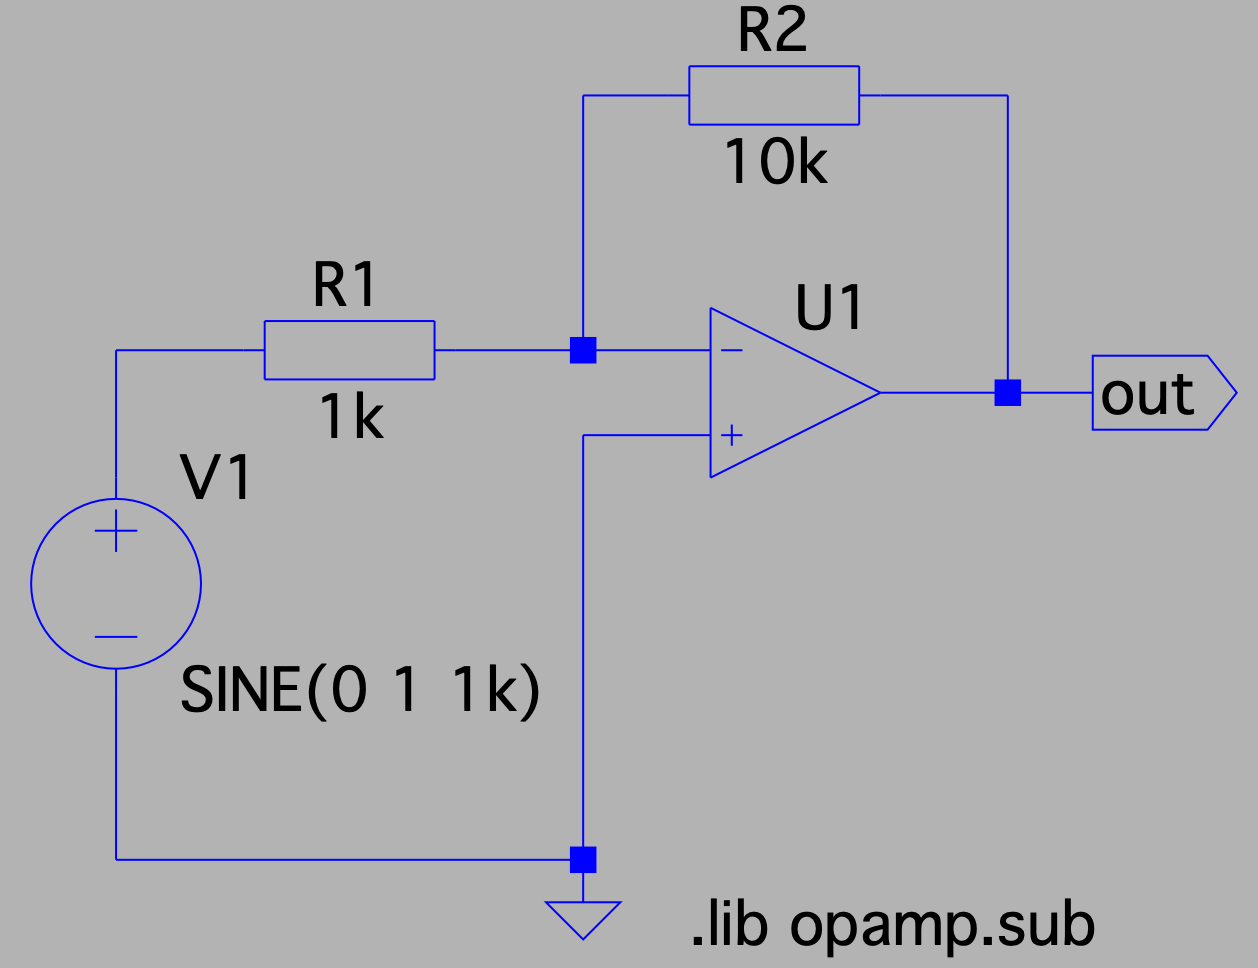
\includegraphics[width=0.8\linewidth]{pictures/opamp_1.png}
          \end{minipage}
                                              &
          \begin{minipage}{.7\textwidth}
            \begin{itemize}
              \item Baut den Schaltplan mit dem o.g. opamp als OPV auf.
              \item Über einen rechten Mausklick kommt ihr ins \textbf{Advanced} Menü der Spannungsquelle. Hier könnt ihr Sie als Signalgenerator konfigurieren. Wir wählen einen \textbf{Sinus mit 1V Amplitude und der Frequenz 1kHz}
              \item Die library kann direkt als spice directive eingebunden werden (siehe Folie 5, .op)
              \item Ihr könnt über die Funktion \textbf{Label Net (F4)} einen Knoten umbennen und ihm mit einem Symbol für In-/Output versehen. Nennt den Ausgang der Schaltung z.B. \textit{out}.
              \item \textbf{Hinweis:} Wenn ihr einen Knoten benennt, dann kann liegt unter diesem Namen überall im Schaltplan das selbe! Potential an.
                    Dadurch könnt ihr den Plan übersichtlicher gestalten.
            \end{itemize}
          \end{minipage}
          \\
                                              & \\
          \hline
        \end{tabular}

      \end{table}

    \end{tiny} \end{spacing}

\end{frame}

\begin{frame}[t]{OPV Schaltungen - transient, ideal}

  \begin{spacing}{0.9} \begin{tiny}
      \begin{table}[h!]
        \begin{tabular}{p{4cm} p{6cm}}
          \hline
          \textbf{Konfiguration der Simulation} & \\
          \hline                                  \\
          \begin{minipage}{.3\textwidth}
            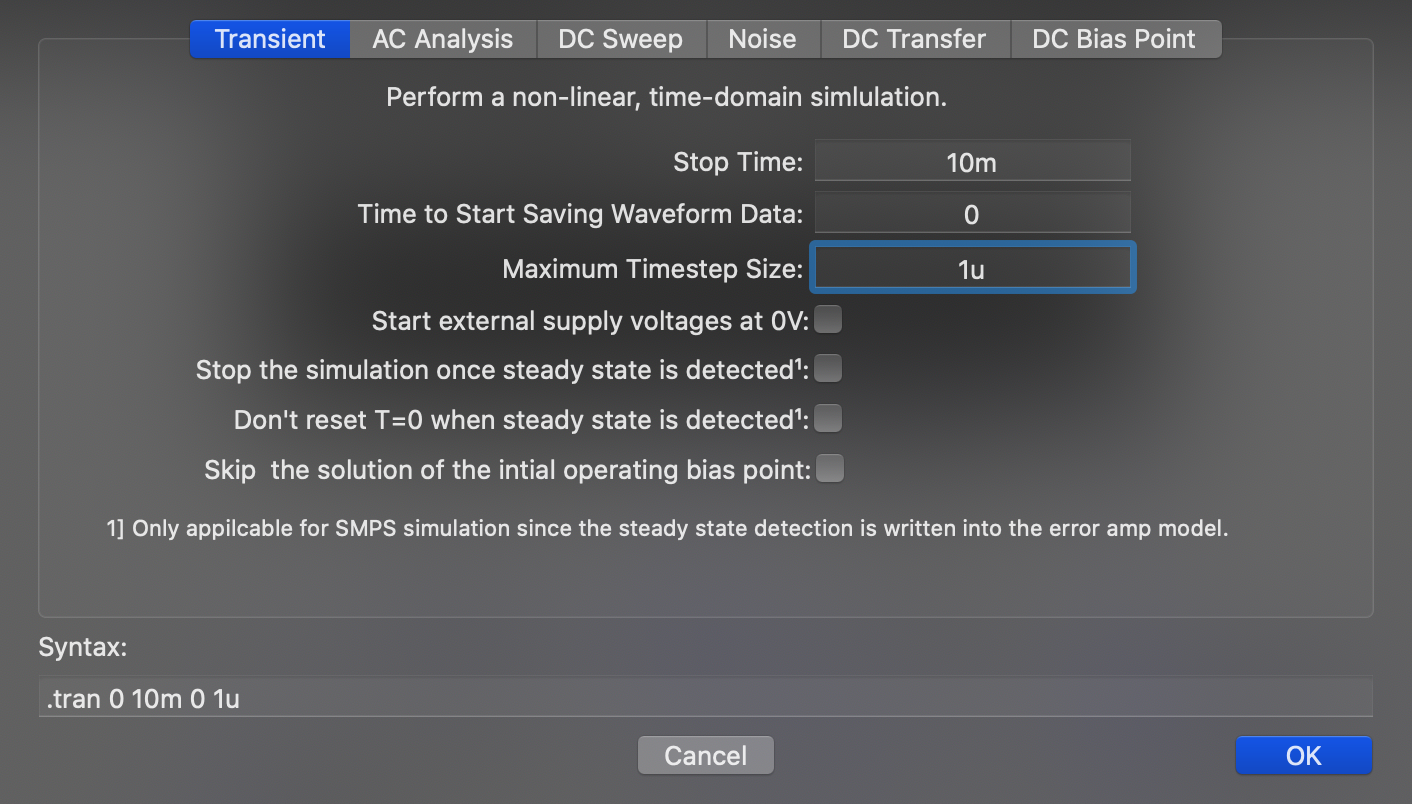
\includegraphics[width=\linewidth]{pictures/simulationcmd_5.png}
          \end{minipage}
                                                &
          \begin{minipage}{.7\textwidth}
            \begin{itemize}
              \item Im Menu Simulation, wählt \textbf{Edit simulation command} und wählt eine \textbf{Transient} Analyse.
              \item Unser Ziel ist es am Ausgang eine Verstärkte Spannung entsprechend des Verstärkungsfaktors der Schaltung zu messen.
              \item Da die Schaltung ideal kein Einschwingverhalten zeigt, starten wir direkt mit der Aufzeichnung und simulieren 10ms mit einer Schrittweite von 10us.
              \item Bestätigt mit \textit{OK} und fügt die Sumlationsansweisung dem schematic hinzu
            \end{itemize}
          \end{minipage}
          \\
                                                & \\
          \hline
          \textbf{Simulation und Analyse}       & \\
          \hline                                  \\
          \begin{minipage}{.5\textwidth}
            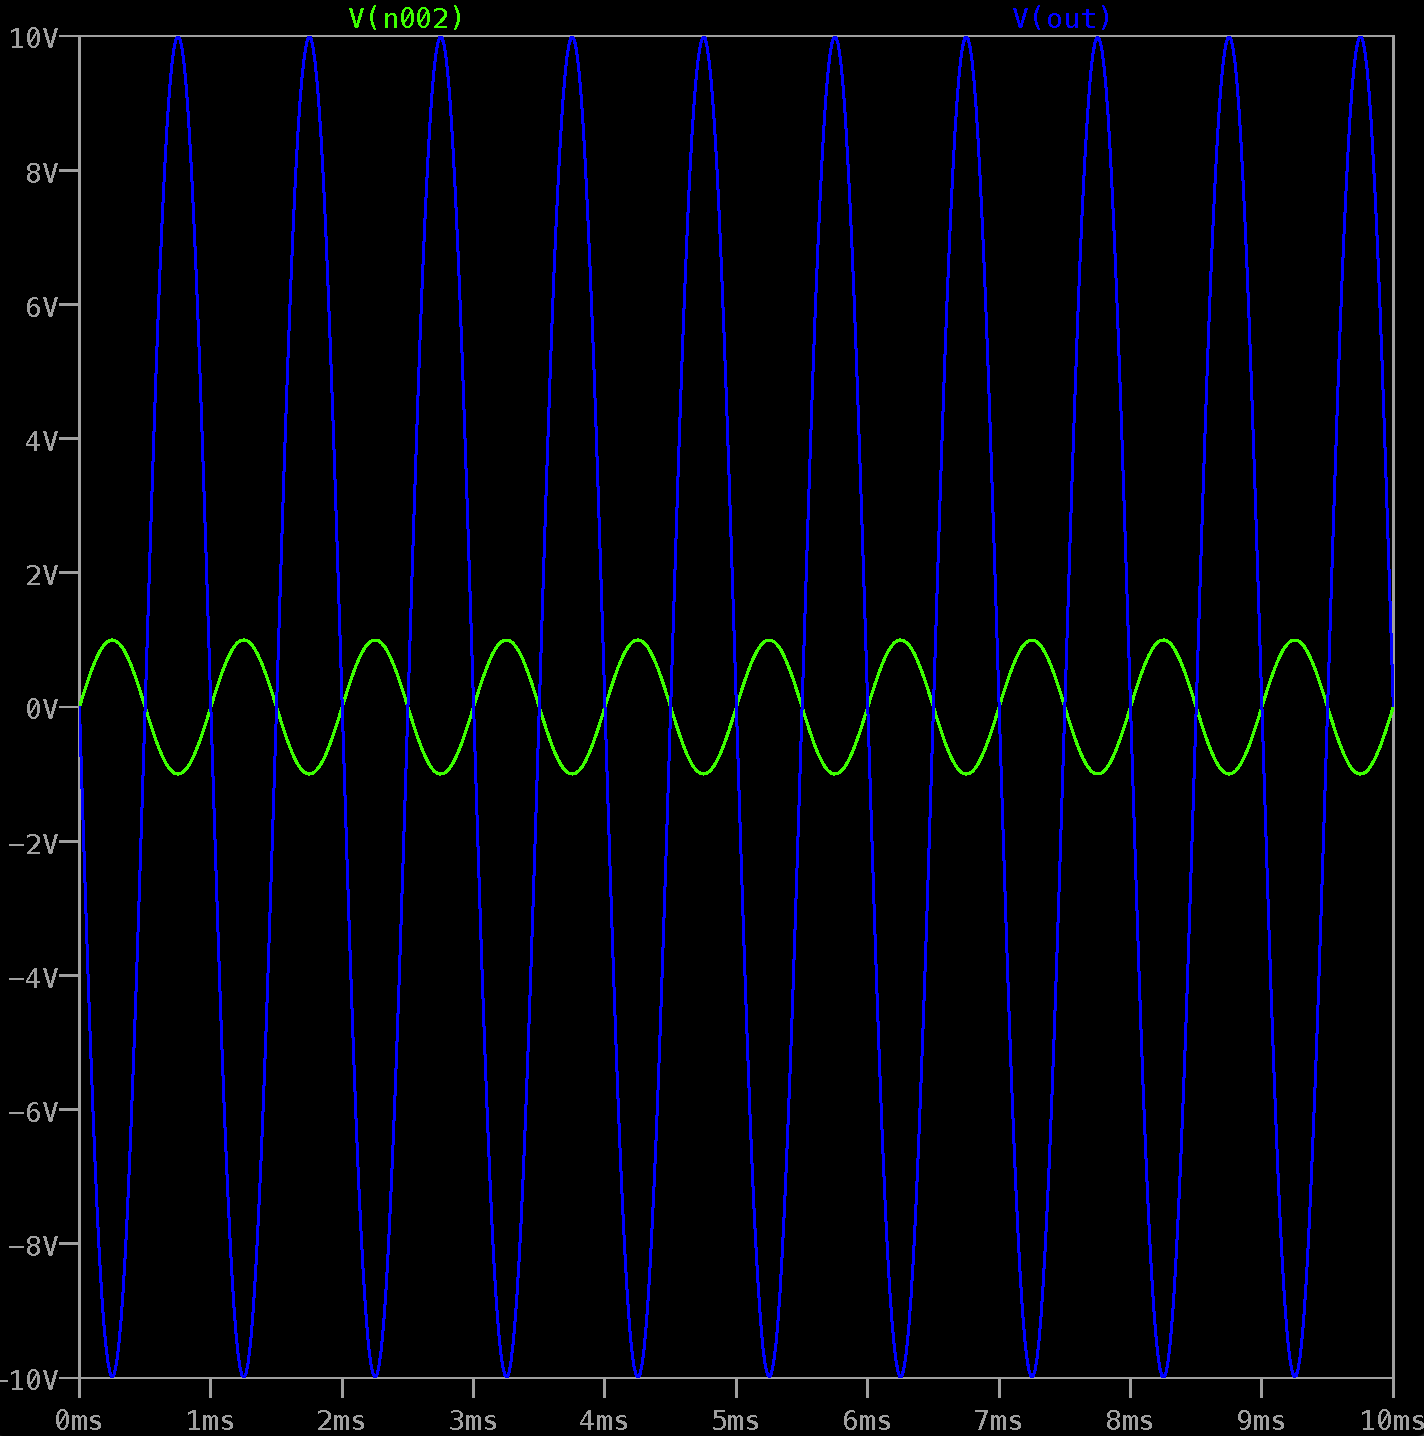
\includegraphics[width=0.5\linewidth]{pictures/analysis_5.png}
          \end{minipage}
                                                &
          \begin{minipage}{.5\textwidth}
            \begin{itemize}
              \item Klickt auf 
\includegraphics[scale=0.3]{pictures/run.png} (run) und LTspice startet die Simulation
              \item Fügt nun die Eingangsspannung sowie die Ausgangsspannung der Schaltung als Messpunkte hinzu.
            \end{itemize}
          \end{minipage}
          \\
        \end{tabular}
      \end{table}
    \end{tiny} \end{spacing}

  \begin{spacing}{0.9} \begin{tiny}
      \begin{table}[h!]
        \begin{tabular}{p{10cm} }
          \hline
          \textbf{Ergebnis und Auswertung} \\
          \hline                           \\
          Verifiziert, ob die Verstärkung sowie das invertierende Verhalten zu eurem Erwartungswert (10) passt.
        \end{tabular}
      \end{table}
    \end{tiny} \end{spacing}

\end{frame}

\begin{frame}[t]{OPV Schaltungen - transient, nicht ideal}

  \begin{spacing}{0.6} \begin{tiny}
      Im nächsten Experiment wollen wir die gleiche Schaltung mit einem "nicht idealen" Verstärken simulieren und die Verwendung
      von Labels verdeutlichen.
    \end{tiny} \end{spacing}

  \begin{spacing}{0.9} \begin{tiny}
      \begin{table}[h!]
        \begin{tabular}{p{3cm} p{7cm}}
          \hline
          \textbf{Erstellung des Schaltplans} & \\
          \hline                                \\
          \begin{minipage}{.3\textwidth}
            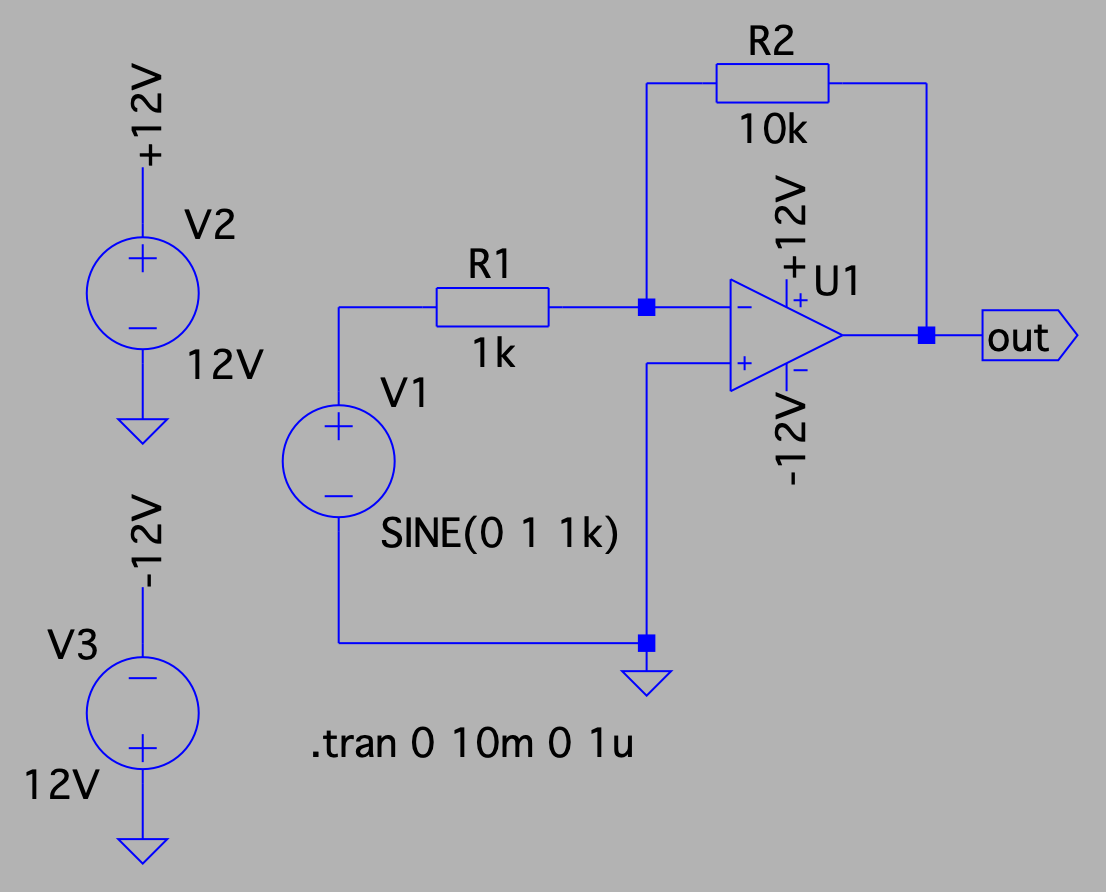
\includegraphics[width=0.8\linewidth]{pictures/opamp_2.png}
          \end{minipage}
                                              &
          \begin{minipage}{.7\textwidth}
            \begin{itemize}
              \item Tauscht den opamp gegen das Bauteil \textbf{UniversalOpamp2} aus dem Bauteileditor (\textbf{F2}).
              \item Fügt zwei neue Spannungsquellen für die Versorgung des OPV's hinzu.
              \item Achtet hierbei auf darauf, dass die Label wirklich auf dem Potential +12V und -12V liegen.
              \item Erstellt die Labels +12V und -12V (\textbf{Label Net (F4)}).
            \end{itemize}
          \end{minipage}
          \\
        \end{tabular}

      \end{table}

    \end{tiny} \end{spacing}


  \begin{spacing}{0.9} \begin{tiny}
      \begin{table}[h!]
        \begin{tabular}{p{10cm} }
          \hline
          \textbf{Ergebnis und Auswertung} \\
          \hline                           \\
          Es muss das selbe Ergebnis herauskommen wie im vorherigen Experiment unter Verwendung des idealen OPV's \textbf{opamp}.
        \end{tabular}
      \end{table}
    \end{tiny} \end{spacing}

\end{frame}


\begin{frame}[t]{OPV Schaltungen - Analyse der Grenzfrequenz einer Schaltung }

  \begin{spacing}{0.6} \begin{tiny}
      Eine Kennzahl von Tief-/Hochpassfiltern ist ihre 3dB Grenzfrequenz $f_g$. Die Grenzfrequenz kann man analytisch, jedoch auch simulativ
      über LTspice bestimmen. Hierzu bietet LTspice die Möglichkeit die Frequenz einer Schaltung zu variieren. Dies wird AC-Sweep genannt.
      Im Bode-Diagramm kann man den logarithmischen Verlauf der Amplitude über der Frequenz in LTspice darstellen und
      somit einfach grafisch die Grenzfrequenz bestimmen indem man den Punkt heraussucht, bei dem die Amplitde um 3dB abgefallen ist.
    \end{tiny} \end{spacing}

  \begin{spacing}{0.9} \begin{tiny}
      \begin{table}[h!]
        \begin{tabular}{p{10cm}}
          \hline
          \textbf{Erstellung des Schaltplans + Konfiguration der Simulation} \\
          \hline
        \end{tabular}
        \begin{tabular}{p{2cm} p{2cm} p{6cm}}
          \begin{minipage}{.2\textwidth}
            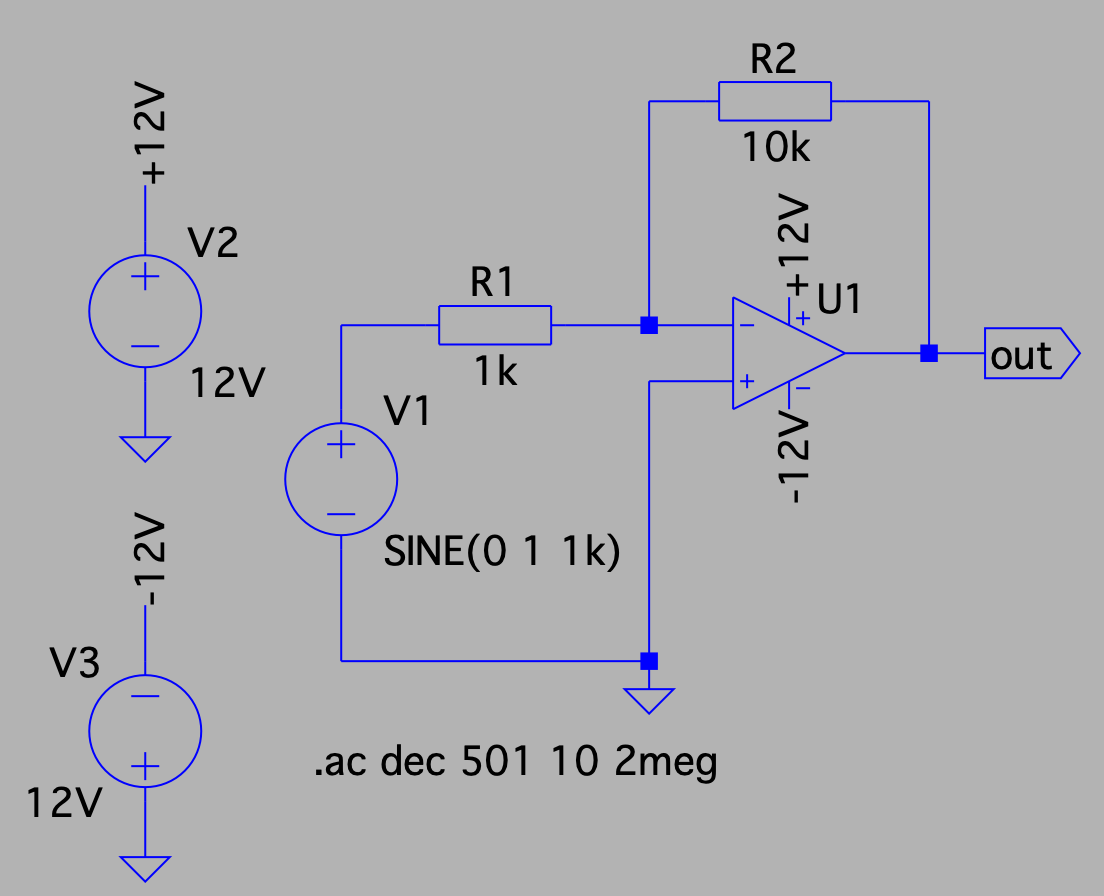
\includegraphics[width=0.8\linewidth]{pictures/opamp_3.png}
          \end{minipage}
           &
          \begin{minipage}{.2\textwidth}
            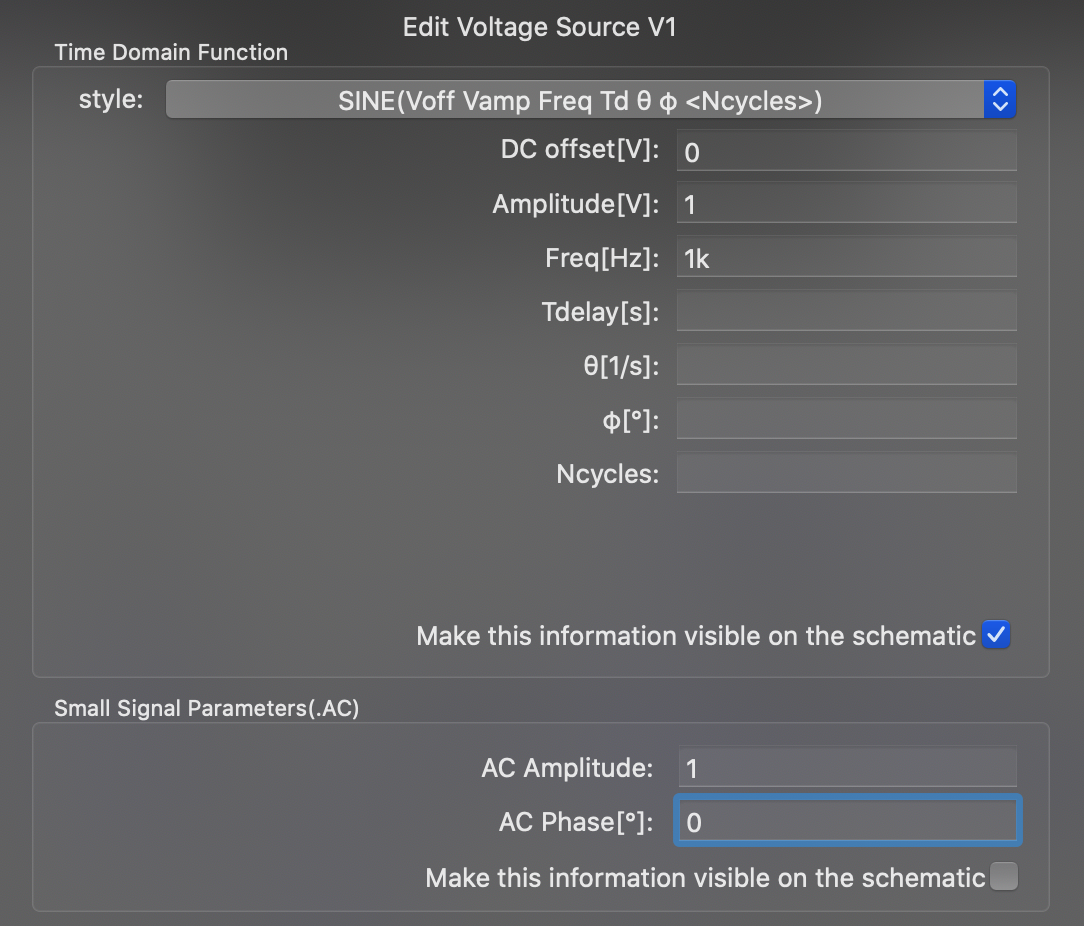
\includegraphics[width=0.8\linewidth]{pictures/ac_small_signal.png}
          \end{minipage}
           &
          \begin{minipage}{.5\textwidth}
            \begin{itemize}
              \item Wir verwenden die Schaltung aus dem vorherigen Beispiel!
              \item Wichtig ist hierbei, dass wir Spannungsquelle für den AC-Sweep konfigurieren
                    Hierzu geht ihr per rechtem Mausklick in das advanced menu von V1 und stellt das Kleinsignal Verhalten (AC)
                    auf \textbf{Amplitude 1V und Frequenz 1kHz}.
            \end{itemize}
          \end{minipage}
          \\
        \end{tabular}
        \begin{tabular}{p{6cm} p{4cm}}
          \hline
          \textbf{Simulation und Analyse} & \\
          \hline                            \\
          \begin{minipage}{.6\textwidth}
            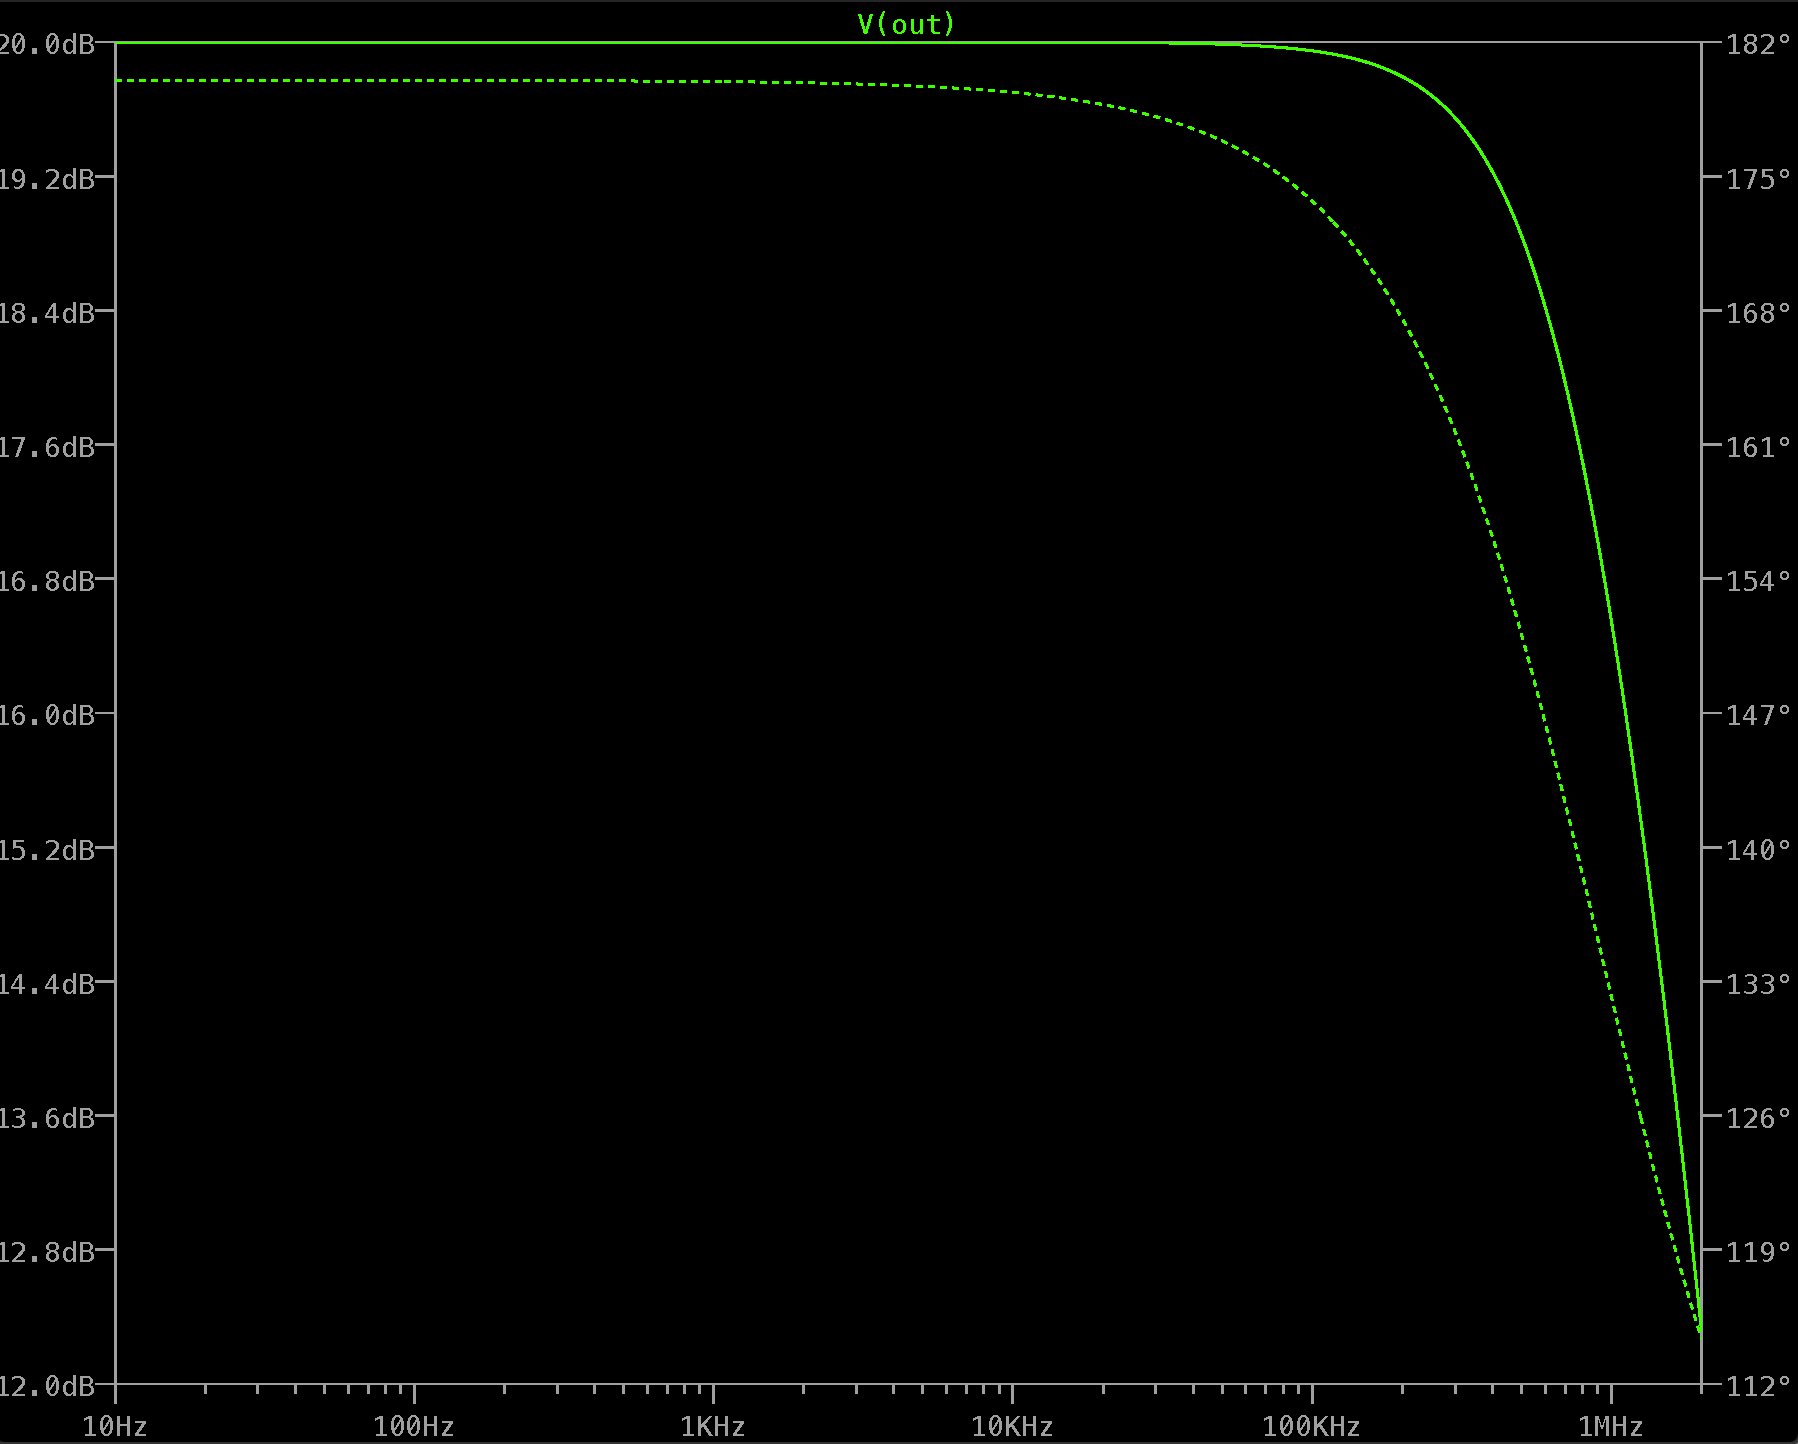
\includegraphics[width=0.7\linewidth]{pictures/analysis_6.png}
          \end{minipage}
                                          &
          \begin{minipage}{.4\textwidth}
            \begin{itemize}
              \item Klickt auf 
\includegraphics[scale=0.3]{pictures/run.png} (run) und LTspice startet die Simulation
              \item Fügt nun die Ausgangsspannung der Schaltung als Messpunkt hinzu.
              \item Im waveform viewer solltet ihr das Bode-Diagram mit Amplitude und Phase sehen.
            \end{itemize}
          \end{minipage}
          \\
        \end{tabular}

      \end{table}

    \end{tiny} \end{spacing}


  %\begin{spacing}{0.9} \begin{tiny}
  %  \begin{table}[h!]
  %    \begin{tabular}{p{10cm} }
  %      \hline
  %      \textbf{Ergebnis und Auswertung} \\
  %      \hline \\    
  %      Es muss das selbe Ergebnis herauskommen wie im vorherigen Experiment unter Verwendung des idealen OPV's \textbf{opamp}.
  %    \end{tabular}
  %  \end{table}
  %\end{tiny} \end{spacing}

\end{frame}

\begin{frame}[t]{OPV Schaltungen - Analyse der Grenzfrequenz einer Schaltung }

  \begin{spacing}{0.9} \begin{tiny}
      \begin{table}[h!]
        \begin{tabular}{p{10cm}}
          \hline
          \textbf{Simulation und Analyse} \\
          \hline                          \\
          \begin{minipage}{\textwidth}
            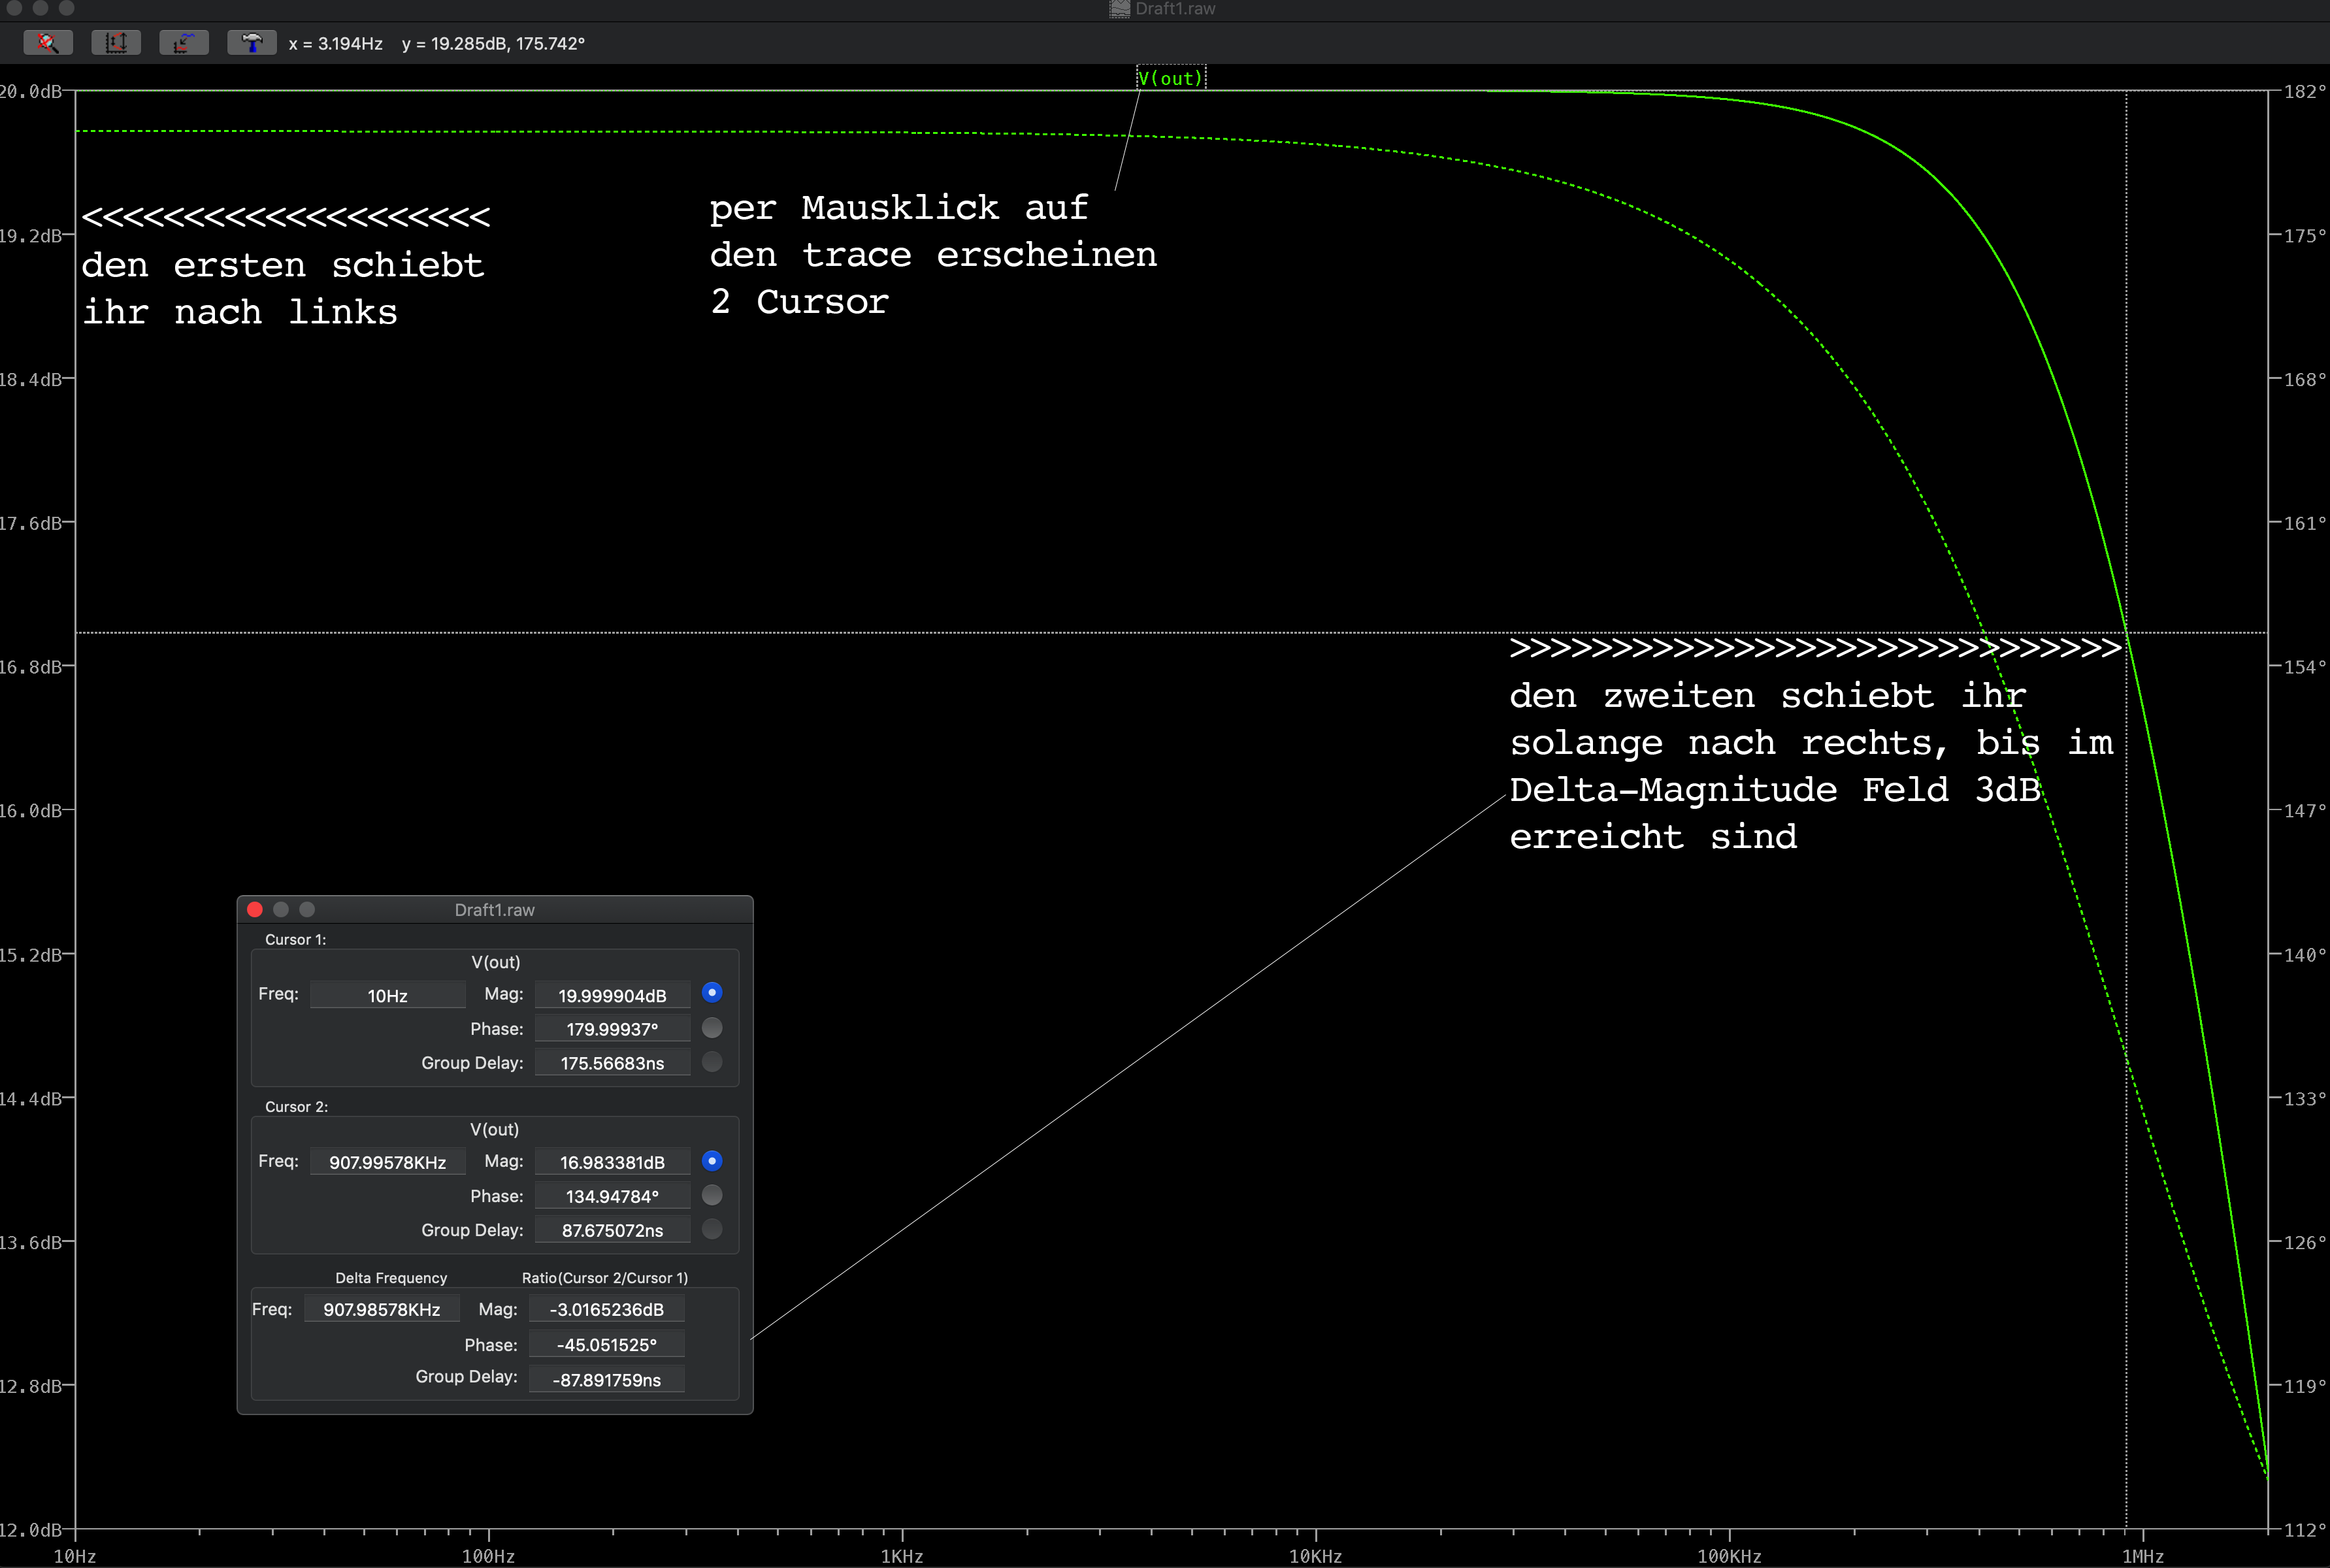
\includegraphics[width=\linewidth]{pictures/bode_1_remastered.png}
          \end{minipage}
          \\
        \end{tabular}

      \end{table}

    \end{tiny} \end{spacing}


  %\begin{spacing}{0.9} \begin{tiny}
  %  \begin{table}[h!]
  %    \begin{tabular}{p{10cm} }
  %      \hline
  %      \textbf{Ergebnis und Auswertung} \\
  %      \hline \\    
  %      Es muss das selbe Ergebnis herauskommen wie im vorherigen Experiment unter Verwendung des idealen OPV's \textbf{opamp}.
  %    \end{tabular}
  %  \end{table}
  %\end{tiny} \end{spacing}

\end{frame}


\begin{frame}[t]{OPV Schaltungen - nicht-invertierender Verstärker}

  \textbf{Ziel - Anwendung der Kenntnisse}

  \begin{spacing}{0.6} \begin{tiny}

      Nachfolgend könnt ihr die Schaltung für einen nicht-invertierenden Verstärker in einer OPV Schaltung sehen.

      \begin{enumerate}
        \item Baut die Schaltung auf, dimensioniert sie so, dass Sie einen Verstärkungsfaktor
        \item Verwendet die UniversalOpamp2 aus der vorherigen Übrung mit einer Versorgungsspannung von +/-12V
        \item Verifiziert eure Schaltung und das \textbf{nicht-invertierende} Verhalten mit einer transienten Simulation von 0 - 50ms.
        \item Wählt dabei eine ausreichend kleine Schrittweite
        \item Wechselt die Simulationsart zum AC-Sweep und ermittelt die Grenzfrequenz
      \end{enumerate}

      \begin{table}[h!]
        \begin{tabular}{p{5cm} p{5cm}}
          \begin{minipage}{.5\textwidth}
            \begin{figure}
              \scalebox{0.35}{
                \centering
                \begin{circuitikz}
                  \ctikzset{bipoles/length=1cm}
                  \draw
                  (0,0) node[op amp,yscale=-1](opamp){}
                  (opamp.+) to[short,-o] ++ (-2,0) to [V=$v_1$] ++ (0,-3) to ++(0,0) node[ground] {}
                  (opamp.-) to[short] ++ (0,-1.25) coordinate(X) to[R,l_=$R_1$] ++(0,-1) node[ground]{}
                  (opamp.out) to[R,l_=$R_2$] ++ (0,-1.5) coordinate(Y) to[short] ++ (-1.7,0) coordinate(X){}
                  (opamp.out) to[short,*-o] ++ (0.5,0) node[right]{$v_{\rm out}$}
                  ;
                \end{circuitikz}
              }

            \end{figure}
          \end{minipage}
           &
          \begin{minipage}{.5\textwidth}
            \begin{equation}
              V_{out}=(1+\frac{R2}{R1})V_{1}
            \end{equation}
          \end{minipage}
        \end{tabular}

      \end{table}

      Spoiler! - Die Lösungen folgen auf den folgenden Folien. Wenn sie sich nicht sicher sind, schauen Sie einfach nach.\newline\newline
      Info! - Besonders die Analyse von Grenzfrequeznen ist für Ihre weitere Vorlesungzeit (Filter höhrerer Ordnung, EMV) hilfreich,
      da Sie neben der simulativen Bestätigung Ihrer Schaltungen auch theoretische Rechenaufgaben simulieren und so Ihre Rechnung
      verifizieren können.

    \end{tiny} \end{spacing}
\end{frame}

\begin{frame}[t]{OPV Schaltungen - Lösung transient}

  \begin{spacing}{0.9} \begin{tiny}
      \begin{table}[h!]
        \begin{tabular}{p{10cm}}
          \hline
          \textbf{Simulation und Analyse} \\
          \hline                          \\
          \begin{minipage}{\textwidth}
            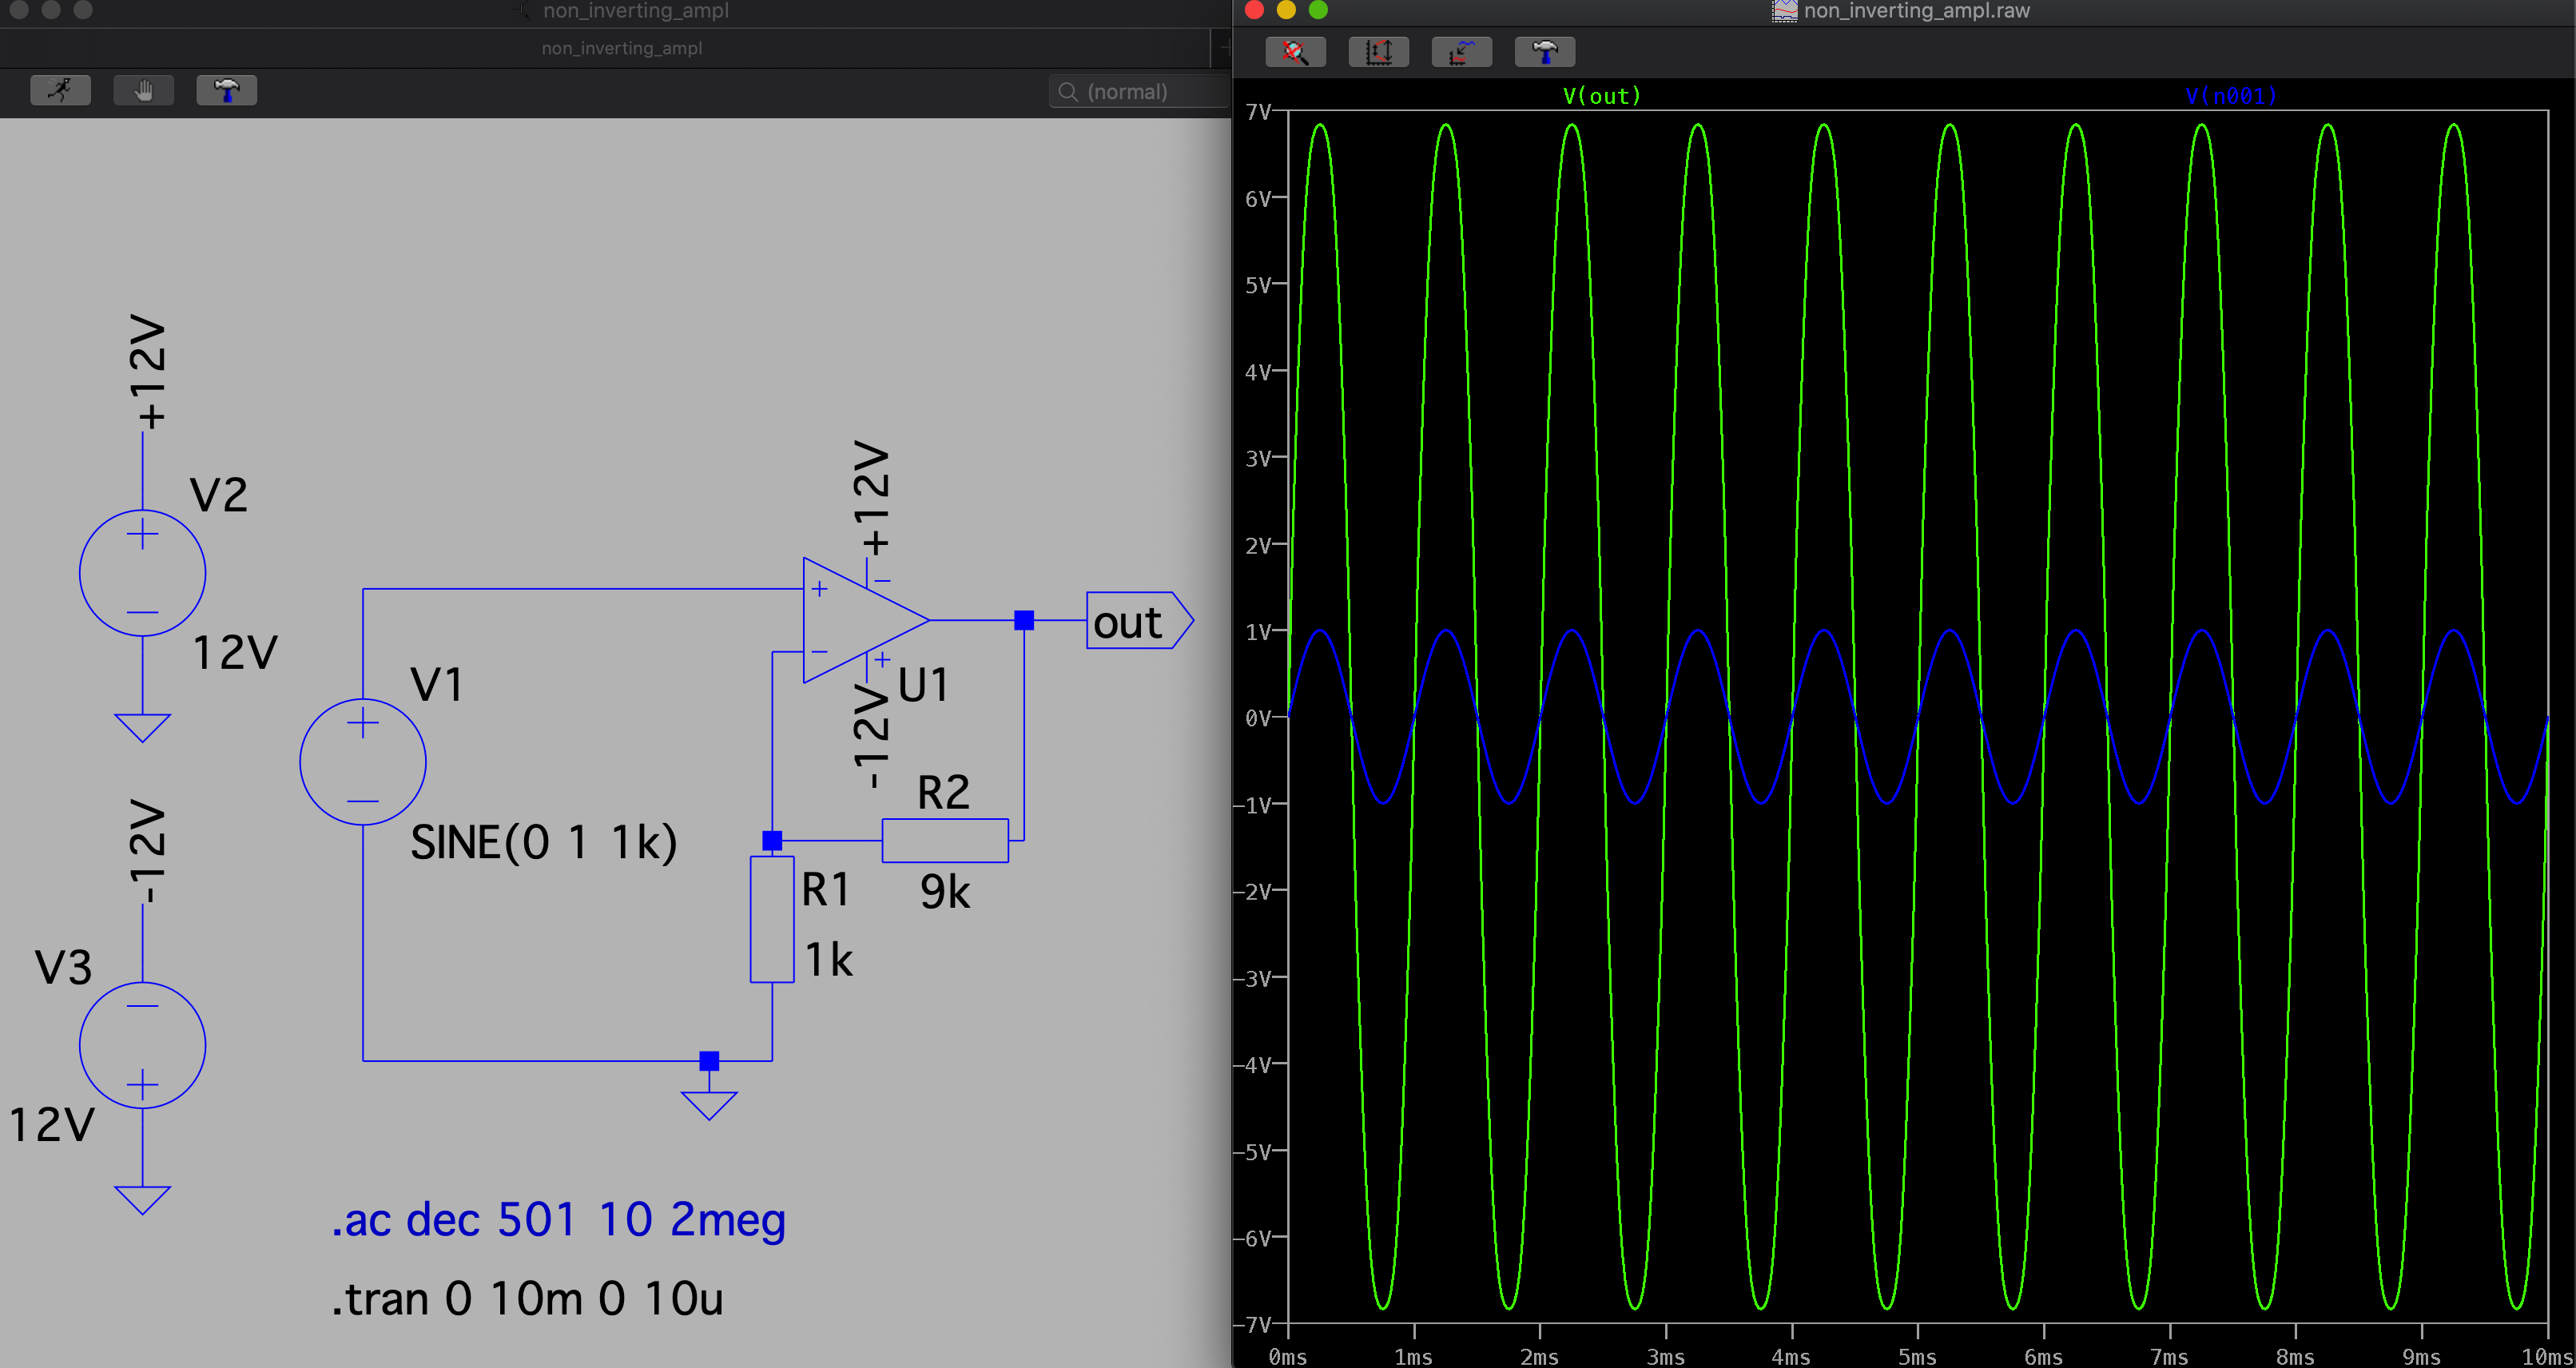
\includegraphics[width=\linewidth]{pictures/analysis_7.png}
          \end{minipage}
          \\
        \end{tabular}

      \end{table}

    \end{tiny} \end{spacing}

\end{frame}

\begin{frame}[t]{OPV Schaltungen - Lösung Grenzfrequenz}

  \begin{spacing}{0.9} \begin{tiny}
      \begin{table}[h!]
        \begin{tabular}{p{10cm}}
          \hline
          \textbf{Simulation und Analyse} \\
          \hline                          \\
          \begin{minipage}{\textwidth}
            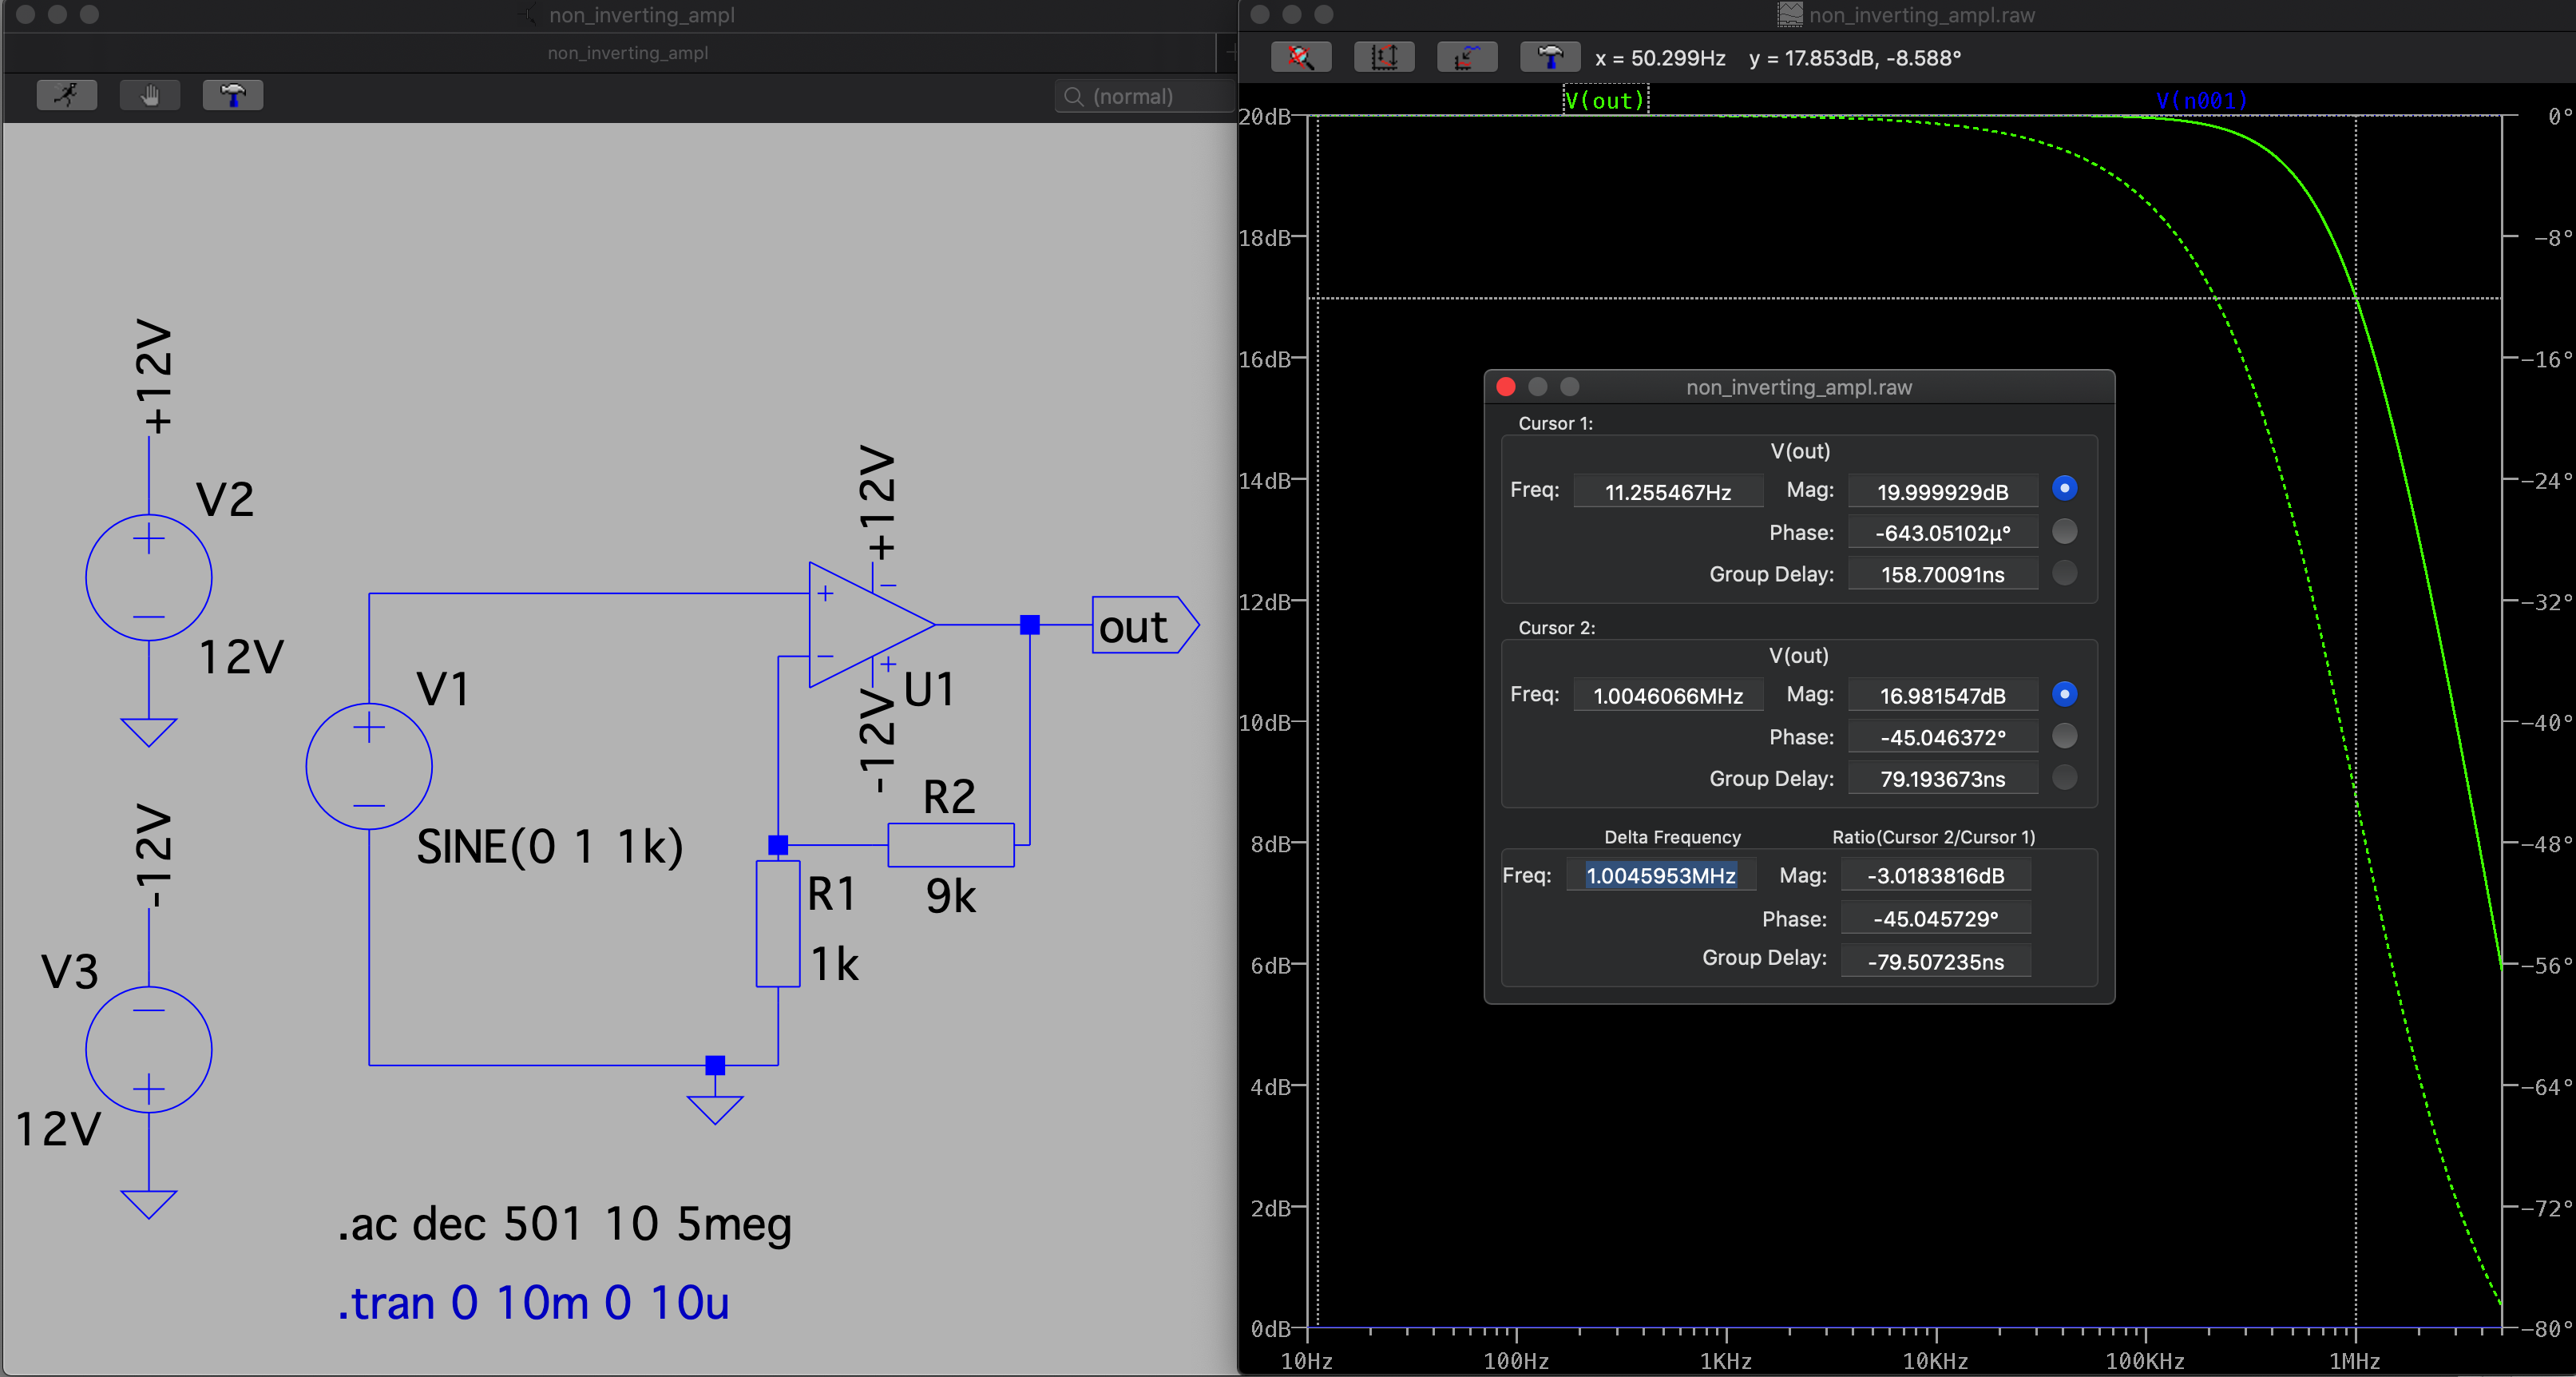
\includegraphics[width=\linewidth]{pictures/bode_2.png}
          \end{minipage}
          \\
        \end{tabular}

      \end{table}

    \end{tiny} \end{spacing}

\end{frame}